\section{Технический проект}

\subsection{Общая характеристика организации решения задачи}

Необходимо спроектировать и разработать программный комплекс для обработки аудиосигналов, сочетающий функциональность профессиональных аудиоредакторов с простотй и удобством интерфейса.

В приложении должно быть:
\begin{itemize}
	\item модульная структура с чётким разделением на: ядро обработки, пользовательский интерфейс, системную обвязку;
	\item гибкая система эффектов: трёхполосный параметрический эквалайзер с настраиваемыми частотами среза, компрессор с регулируемыми параметрами, алгоритм реверберации;
	\item оптимизированная обработки сигнала: поддержка многопоточной обработки для работы в реальном времени, аппаратно-независимая реализация звукового движка, автоматическая нормализация входного и выходного сигнала;
	\item интерактивная визуализация; формы волны во временной области, АЧХ применяемых фильтров.
\end{itemize}
 
\subsection{Обоснование выбора технологий проектирования}

Используемые для создания программно-информационной системы языки и технологии отвечают современным практикам разработки, позволяют достичь высокой производительности и отказоустойчивости программы.

\subsubsection{Язык программирования Python}

Python - основной язык разработки проекта. Python выбран благодаря своей гибкости, богатой экосистеме библиотек и кроссплатформенной поддержке. Его синтаксис позволяет быстро разрабатывать сложные алгоритмы обработки сигналов, а динамическая типизация упрощает интеграцию с различными аудиоформатами и устройствами.

Используемые библиотеки:
\begin{itemize}
	\item NumPy - обеспечивает высокопроизводительные вычисления с многомерными массивами, что критично для обработки аудиоданных, представленных в виде временных рядов;
	\item SciPy - используется для реализации цифровых фильтров (эквалайзер), БПФ (анализ спектра) и других математических операций;
	\item PyDub - библиотека для работы с аудиофайлами, предоставляющая: простые методы загрузки и сохранения в форматах WAV, MP3, OGG, FLAC, базовые операции, такие как обрезка, наложение, изменение громкости, конвертация частоты дискретизации, интеграцию с FFmpeg для поддержки дополнительных кодеков;
	\item SoundDevice - обеспечивает низкоуровневый доступ к аудиоустройствам через PortAudio. Ключевые функции: воспроизведение и запись в реальном времени с минимальной задержкой, поддержка ASIO, WASAPI, Core Audio для профессиональных аудиоинтерфейсов, гибкая настройка параметров потока: частота дискретизации, размер буфера, количество каналов;
	\item Matplotlib - используется для визуализации аудиоданных: построение осциллограмм (форма сигнала во временной области), отображение АЧХ (амплитудно-частотных характеристик) с логарифмической шкалой, интерактивное обновление графиков в реальном времени;
	\item Tkinter - стандартная библиотека Python для создания графического интерфейса. В проекте применяется для: построения основного окна с вкладками (эквалайзер, компрессор, реверберация), реализации интерактивных элементов: ползунки, кнопки, метки, интеграции графиков Matplotlib через FigureCanvasTkAgg;
	\item Numba - JIT-компилятор для оптимизации вычислительно сложных участков кода: ускорение алгоритмов компрессии и реверберации в 5–10 раз, поддержка многопоточности.
\end{itemize}

\subsubsection{Кроссплатформенная библиотека FFmpeg}

FFmpeg — это мощная кроссплатформенная библиотека для обработки мультимедиа, используемая в проекте для работы с аудиофайлами различных форматов. Взаимодействие с FFmpeg осуществляется через обёртку PyDub, что значительно упрощает операции чтения, записи и конвертации аудио.

Основные функции FFmpeg в проекте:
\begin{enumerate}
	\item Поддержка множества аудиоформатов. Позволяет загружать и сохранять файлы в форматах: без сжатия: WAV, AIFF, с потерями: MP3, AAC, OGG, без потерь: FLAC, ALAC. Обеспечивает автоматическое определение кодека при загрузке.
	\item Конвертация аудио: изменение частоты дискретизации, преобразование между форматами, конвертация числа каналов.
	\item Нормализация и обработка. Автоматическая регулировка громкости.
\end{enumerate}

FFmpeg был выбран по рядам преимуществ:
\begin{itemize}
	\item универсальность: поддержка 100+ кодеков и контейнеров;
	\item стабильность: отлаженные алгоритмы декодирования/кодирования;
	\item производительность: оптимизированные нативные библиотеки;
	\item гибкость: Возможность тонкой настройки параметров через командные опции.
\end{itemize}

\subsection{Эффекты}

\subsubsection{Устройство эквалайзера}

Эквалайзер — это устройство или программный алгоритм, предназначенный для корректировки амплитудно-частотной характеристики (АЧХ) звукового сигнала. Он позволяет усиливать или ослаблять определённые частотные диапазоны, изменяя тембр звука. Эквалайзер работает, разделяя входной аудиосигнал на несколько частотных полос (диапазонов), каждая из которых обрабатывается отдельно. После обработки всех полос сигналы складываются, и на выходе получается звук с изменённой частотной характеристикой.

В программе реализован цифровой параметрический эквалайзер, у которого есть три полосы частот, а так же коррекция их по громкости в децибелах. Такие эквалайзеры часто используются в профессиональной звукозаписи и сведении аудио.

Цифровой IIR-фильтр (Биквадратный, на основе Баттерворта)

IIR-фильтр (Infinite Impulse Response — бесконечная импульсная характеристика) — это тип цифрового фильтра, который использует обратную связь, благодаря чему может иметь очень крутые склоны АЧХ при малом порядке.

Биквадратный фильтр (Biquad) — это частный случай IIR-фильтра 2-го порядка, который реализуется с помощью разностного уравнения и часто используется в эквалайзерах из-за своей эффективности.

Фильтр Баттерворта — один из самых популярных типов фильтров, обеспечивающий максимально гладкую АЧХ в полосе пропускания без пульсаций.

Этот эквалайзер обеспечивает:
\begin{itemize}
	\item низкую задержку (важно для реального времени);
	\item минимальные фазовые искажения;
	\item точную обработку частот;
	\item защиту от перегрузки.
\end{itemize}

\subsubsection{Устройство компрессора}

Feed-forward компрессор — это тип динамического процессора, в котором уровень входного сигнала анализируется до применения gain reduction, что позволяет более точно контролировать амплитудные изменения. В сочетании с RMS-детектированием огибающей такой компрессор обеспечивает плавное и музыкальное сжатие, идеально подходящее для обработки вокала, гитар и других сложных сигналов с выраженными динамическими перепадами.

RMS (Root Mean Square) — среднеквадратичное значение сигнала, которое лучше отражает воспринимаемую громкость, чем пиковый уровень (Peak). На практике RMS вычисляется с использованием скользящего среднего или фильтра низких частот (ФНЧ) для сглаживания.

Основные этапы обработки:
\begin{itemize}
	\item входной сигнал поступает на детектор огибающей;
	\item RMS-детектор вычисляет усреднённый уровень сигнала;
	\item порог (Threshold) определяет момент начала компрессии;
	\item коэффициент сжатия (Ratio) задаёт силу уменьшения уровня;
	\item временные параметры (Attack/Release) регулируют скорость реакции;
	\item Make-up Gain компенсирует потерянную громкость.
\end{itemize}

Ключевые особенности:
\begin{itemize}
	\item плавность: RMS-детектирование снижает резкость обработки по сравнению с Peak;
	\item гибкость: Attack/Release настраиваются отдельно для атаки и восстановления;
	\item применение: вокал, живые инструменты, мастер-каналы.
\end{itemize}

\subsubsection{Устройство реверберации}

FDN (Feedback Delay Network) — это один из самых мощных алгоритмов цифровой реверберации, используемый для создания реалистичных пространственных эффектов. Он основан на множестве линий задержки с обратной связью, образующих сложную сеть, имитирующую отражения в помещении.

Принцип работы:
\begin{itemize}
	\item входной сигнал разделяется на несколько параллельных линий задержки, каждая из которой задерживает сигнал на разное время;
	\item после задержки сигнал проходит через фильтр демпфирования (имитация потери высоких частот);
	\item затем он умножается на коэффициенты матрицы обратной связи, определяющей, какая часть сигнала возвращается в каждую линию;
	\item обновлённый сигнал снова поступает на вход линий задержки;
	\item результирующий реверберационный сигнал формируется как сумма выходов всех линий.
\end{itemize}

Ключевые особенности FDN:
\begin{itemize}
	\item реалистичность — лучше имитирует поздние отражения, чем алгоритмы на основе простых задержек;
	\item гибкость — можно настраивать время реверберации, демпфирование и пространственность;
	\item стабильность — ортогональная матрица гарантирует отсутствие бесконечного нарастания.
\end{itemize}

\subsection{Архитектура программной системы}

На рисунке \ref{DiagramArch:image} представлена многослойная архитектура системы с чётким разделение ответственности между компонентами.

\begin{figure}[p]  % Разместить на отдельной странице
	\centering
	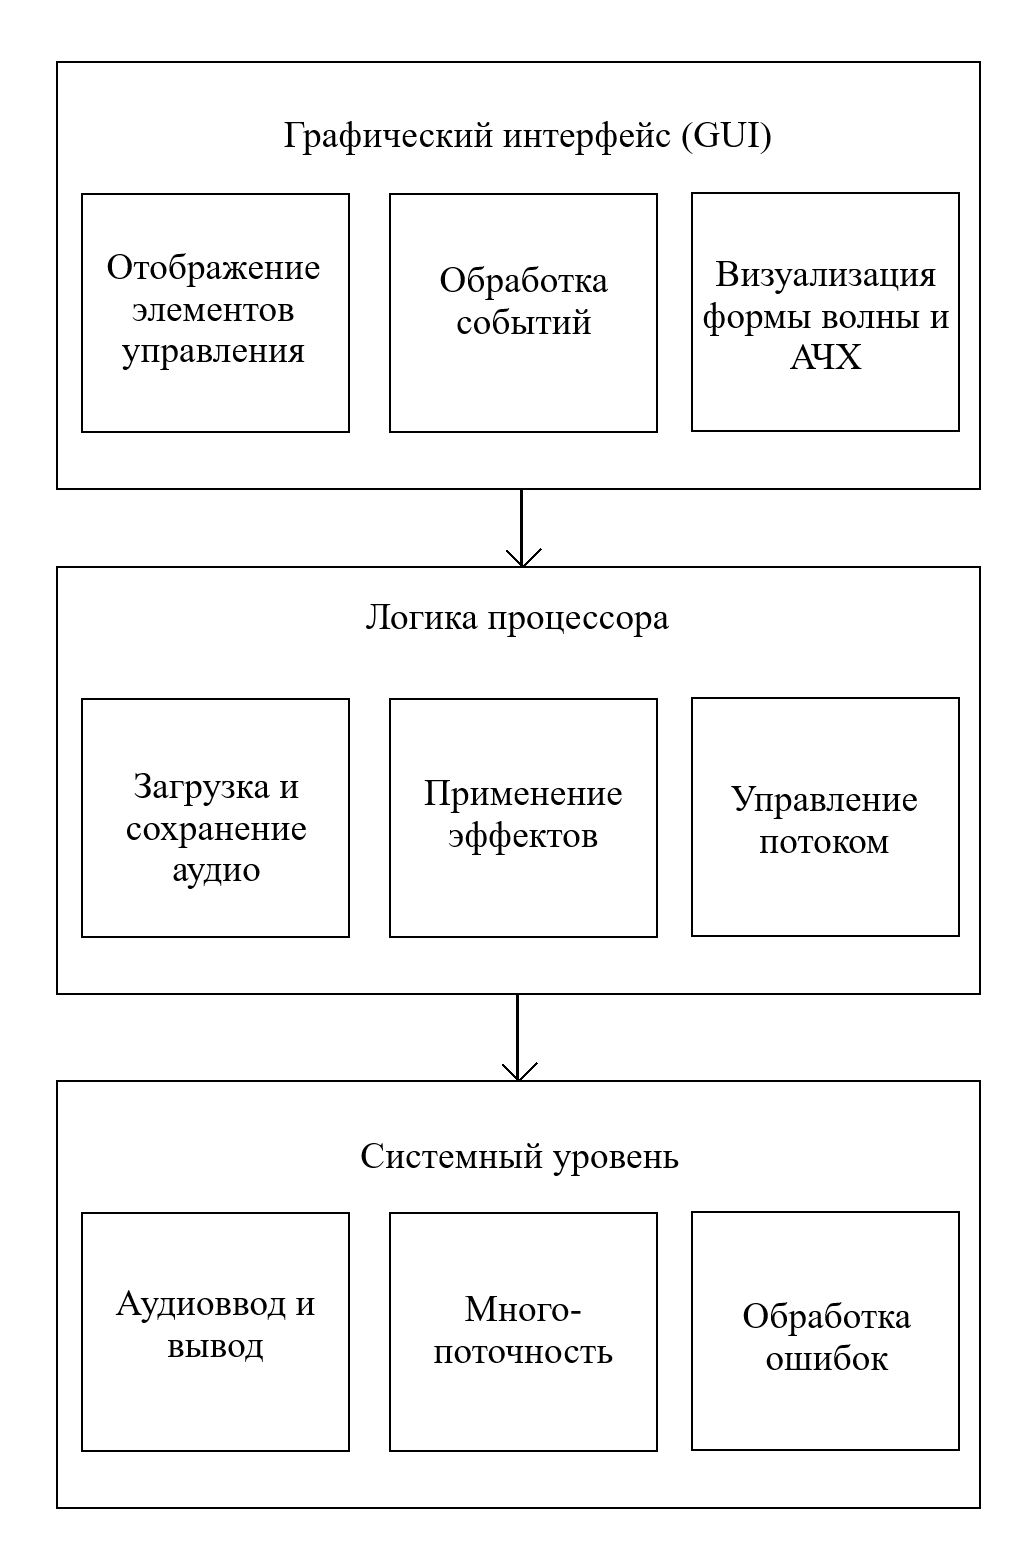
\includegraphics[width=0.8\linewidth]{DiagramArch}
	\caption{Архитектура программной системы}
	\label{DiagramArch:image}
\end{figure}
\clearpage

\begin{enumerate}
	\item Графический интерфейс отображает элементы управления (кнопки, ползунки, вкладки), визуализирует аудиоданные в реальном времени (Осциллограмма, АЧХ), обрабатывает пользовательские события (нажатия кнопок, изменение параметров).
	\item Логика процессора отвечает за загрузку/сохранение аудио, чтение файлов через PyDub/FFmpeg, конвертирует в формат float32 для обработки. Применяет эффекты: эквалайзер (БИХ-фильтры для НЧ/СЧ/ВЧ), компрессор (динамическое сжатие с параметрами), реверберация. Буферизирует данные и синхронизирует позицию воспроизведения.
	\item На уровне системы происходит ввод и вывод аудио, создаётся отдельный поток для обработки аудио и очереди для передачи данных между потоками. Обрабатываются ошибки, перехватываются исключения и логируются в файл.
\end{enumerate}

\subsection{Компоненты программы}

Приложение Audio Processor состоит из следующих ключевых компонентов, организованных в модульную структуру:
\begin{itemize}
	\item графический интерфейс включает главное окно, состоящее из кнопок управление воспроизведением и загрузки/сохранения, вкладок эффектов (эквалайзер, компрессор и ревербератор), окна отображение визуализации формы волны и АЧХ;
	\item логика процессора читает и обрабатывает аудиофайлы, применяется выбранные эффекты по очереди, управляет всей работой программы;
	\item системное устройство воспроизводит звук, работает с файлами, открывает и сохраняет их, управляет несколькими задачами одновременно;
	\item вспомогательные модули включают частотный анализ, автоматически регулирует громкость и записывает ошибки и события.
\end{itemize}

Все части программы взаимодействуют между собой по чётким правилам. Когда пользователь меняет настройки, интерфейс передаёт их в модуль обработки, который применяет эффекты и отправляет результат на воспроизведение и отображение. Для плавной работы использовались очереди задач для работы в многопоточном режиме, оптимизирует сложные вычисления для быстрой работы.

\subsection{Архитектура приложения}
Приложение построено по многослойной модульной архитектуре с разделением на логические компоненты, взаимодействующие через четко определенные интерфейсы. В основе лежит ядро обработки аудиосигналов, окруженное графическим интерфейсом, системными сервисами и вспомогательными модулями.
Графический интерфейс реализован на Tkinter и включает:
\begin{itemize}
	\item главное окно (MainWindow) с вкладками для управления эффектами, кнопками воспроизведения/паузы и областью визуализации;
	\item панель эквалайзера (EQPanel) с тремя ползунками (НЧ/СЧ/ВЧ), отображающая АЧХ через Matplotlib;
	\item панель компрессора (CompressorPanel) для настройки порога, сжатия, атаки, восстановления, усиления;
	\item панель реверберации (ReverbPanel) для настройки эффект, сухой сигнал, размер комнаты, затухание;
	\item визуализатор спектра (SpectrumAnalyzer), отображающий осциллограмму (форма сигнала) и частотный спектр (БПФ) в реальном времени;
	\item прогресс-бар с управлением позицией воспроизведения и отображением длительности трека.	
\end{itemize}

Логический процессор — центральный модуль, отвечающий за:
\begin{itemize}
	\item загрузку и конвертацию аудио через PyDub (с использованием FFmpeg как бэкенда), включая поддержку WAV, MP3, FLAC;
	\item эквалайзер на БИХ-фильтрах с частотами 150 Гц (НЧ), 1 кГц (СЧ), 5 кГц (ВЧ);
	\item компрессор с параметрами knee, makeup gain;
	\item реверберация на основе алгоритма Schroeder (комбинация линий задержки и FIR-фильтров);
	\item буферизацию данных для плавного воспроизведения и нормализацию уровня сигнала.
\end{itemize}

Системный слой обеспечивает интеграцию с ОС и оборудованием:
\begin{itemize}
	\item аудиопоток (AudioStream) на базе SoundDevice, обрабатывающий ввод/вывод в реальном времени с настройкой latency и sample rate (44.1–192 кГц);
	\item менеджер потоков (ThreadManager) для параллельной обработки (отдельные потоки для: GUI, аудиообработки, визуализации);
	\item файловый менеджер (FileManager) с кэшированием загруженных треков и поддержкой метаданных (ID3-теги).
\end{itemize}

Архитектура обеспечивает масштабируемость (добавление новых эффектов через модули), производительность (JIT-компиляция, многопоточность) и отказоустойчивость (изоляция сбоев в отдельных потоках).

\subsection{Проект данных программной системы}

Система оперирует тремя основными категориями данных: входными, промежуточными и выходными. Входные данные включают аудиофайлы в форматах WAV, MP3, FLAC и OGG с поддержкой различных характеристик (битность 16-24 бит, частота дискретизации 44.1-192 кГц), а также параметры эффектов, настраиваемые пользователем через графический интерфейс. Для эквалайзера это уровни усиления по трём полосам (низкие на 150 Гц, средние на 1 кГц, высокие на 5 кГц с диапазоном ±24 дБ), для компрессора — порог срабатывания от -60 до 0 дБ, коэффициент компрессии от 1:1 до 20:1, время атаки и восстановления от 0.1 до 500 мс, для реверберации — соотношение обработанного и исходного сигнала, коэффициент затухания и виртуальный размер помещения.

Промежуточные данные представлены в виде нормализованных аудиобуферов в формате 32-битных чисел с плавающей запятой, организованных как моно- или стереоканальные массивы. Система использует кольцевые буферы для обработки в реальном времени и промежуточные спектральные данные, полученные через быстрое преобразование Фурье с применением оконной функции. Для хранения состояния эффектов используются специализированные структуры: коэффициенты БИХ-фильтров эквалайзера, параметры огибающей компрессора и линии задержки реверберации.

Выходные данные включают обработанные аудиофайлы в выбранных пользователем форматах (WAV с PCM-кодированием или MP3 с переменным битрейтом), сохраняющие исходные параметры частоты дискретизации или конвертируемые к стандартным значениям. Визуализационные данные содержат три основных компонента: осциллограмму последних обработанных сэмплов, частотный спектр с разрешением 8192 точек и амплитудно-частотную характеристику активных фильтров, отображаемую в логарифмическом масштабе от 20 Гц до 20 кГц.

Метаданные системы включают пользовательские пресеты эффектов, содержащие полный набор параметров обработки, историю операций для возможности отмены действий, а также технические лог-файлы с информацией о производительности и ошибках. Все данные передаются между компонентами системы через единый формат аудиоблоков, сопровождаемых метаинформацией о текущих настройках обработки, что обеспечивает согласованность работы многопоточной архитектуры.

\subsubsection{Описание сущностей графического интерфейса}

Графический интерфейс Audio Processor представляет собой комплекс взаимосвязанных визуальных компонентов, объединенных в единое интуитивное пространство. 

Интерфейс поддерживает несколько режимов отображения - компактный для мониторов с малым разрешением, расширенный с дополнительными инструментами анализа для профессиональной работы, и режим презентации с увеличенными элементами управления. Все визуальные компоненты реализованы с учетом эргономики - важные элементы выделены акцентным цветом, соблюдены принципы визуальной иерархии, обеспечена последовательная реакция на пользовательские действия. Особенностью интерфейса является синхронизация всех элементов - изменения параметров эффектов мгновенно отражаются на графиках, а действия пользователя сопровождаются тактильной обратной связью в виде тонких анимационных эффектов.

\subsubsection{Описание сущностей логики процессора}

Основу обработки составляет низкоуровневый модуль, работающий с потоком аудиосэмплов в формате 32-битных чисел с плавающей точкой, обеспечивающий базовые операции нормализации и передискретизации. Система эффектов построена вокруг трех ключевых процессоров: эквалайзер реализует трехполосную фильтрацию через каскад БИХ-фильтров с настраиваемыми частотами среза и коэффициентами усиления, компрессор отвечает за компрессию сигнала с алгоритмами расчета огибающей и адаптивными параметрами атаки/восстановления, а ревербератор генерирует реверберацию через комбинацию линий задержки с регулируемыми параметрами затухания.

Поток данных управляется специализированным менеджером маршрутизации, который обеспечивает передачу аудиоблоков между модулями с минимальной задержкой, используя кольцевые буферы и механизм синхронизации для многопоточной работы. Состояние системы отслеживает активные эффекты, параметры обработки и текущий режим работы (реальное время/оффлайн обработка), предоставляя единый интерфейс для управления конвейером обработки. 

\subsubsection{Описание сущностей системного уровня}

Системная архитектура приложения построена на нескольких ключевых компонентах, обеспечивающих интеграцию с операционной средой и аппаратными ресурсами. Центральным элементом выступает абстрактный слой взаимодействия с аудиодрайверами, реализующий поддержку ASIO, WASAPI и Core Audio через единый кроссплатформенный API. Для управления устройствами ввода-вывода используется DeviceManager, который автоматически обнаруживает доступные аудиоинтерфейсы, анализирует их характеристики и предоставляет унифицированный интерфейс для работы с ними.

Файловая подсистема основана на компоненте, объединяющем возможности стандартных Python-библиотек для работы с файлами и мощь FFmpeg для обработки мультимедиа. Этот модуль включает кэширующий механизм для ускорения повторного доступа к аудиофайлам и систему контроля целостности данных. 

Многопоточная архитектура координируется центральным диспетчером задач, который создает и управляет тремя основными типами потоков: высокоприоритетным аудиопотоком реального времени, фоновыми рабочими потоками для обработки эффектов и служебными потоками для визуализации и логирования.

\subsection{Проектирования пользовательского интерфейса}

Центральное место занимает динамическая визуализация аудиопотока - двойной дисплей с синхронизированными осциллограммой и АЧХ, выполненный в темной цветовой гамме с акцентными элементами салатового цвета для выделения ключевых параметров сигнала. Основная рабочая область: верхняя треть экрана отведена под графики, центральная часть содержит компактные панели эффектов с интуитивными регуляторами, а нижний сектор занимает расширенная панель транспорта с профессиональными элементами управления.

Навигационная система реализована через адаптивную панель вкладок с контекстно-зависимыми элементами управления - при выборе конкретного эффекта (эквалайзер, компрессор, реверберация) нижняя панель автоматически наполняется соответствующими регуляторами, сохраняя при этом быстрый доступ к основным функциям. Все элементы управления спроектированы с учетом тактильного взаимодействия - ползунки имеют выраженные рифленые ручки с магнитными точками для часто используемых значений, кнопки обладают трехступенчатой визуальной обратной связью (покой, наведение, нажатие), а переключатели сопровождаются мягкими анимационными переходами.

На рисунке 3.2 представлен интерфейс программы при запуске. Макет содержит следующие элементы:
\begin{enumerate}
	\item Окно вывода графика формы волны.
	\item Окно вывода АЧХ.
	\item Активная кнопка для загрузки аудио.
	\item Активная кнопка для воспроизведения аудио.
	\item Не активная кнопка для остановки аудио.
	\item Не активная кнопка для сохранения аудио.
	\item Вкладка выбора эффекта эквалайзер (выбран).
	\item Вкладка выбора эффекта компрессор (не выбран).
	\item Вкладка выбора эффекта реверберации (не выбран).
	\item Бегунок регулировки низких частот.
	\item Бегунок регулировки средних частот.
	\item Бегунок регулировки высоких частот.
	\item Чекбокс включения эквалайзера.
	\item Бегунок управления временем начала воспроизведения.
	\item Время, в которое воспроизводится аудио и полная длина файла.
\end{enumerate}

\begin{figure}[ht]
	\center{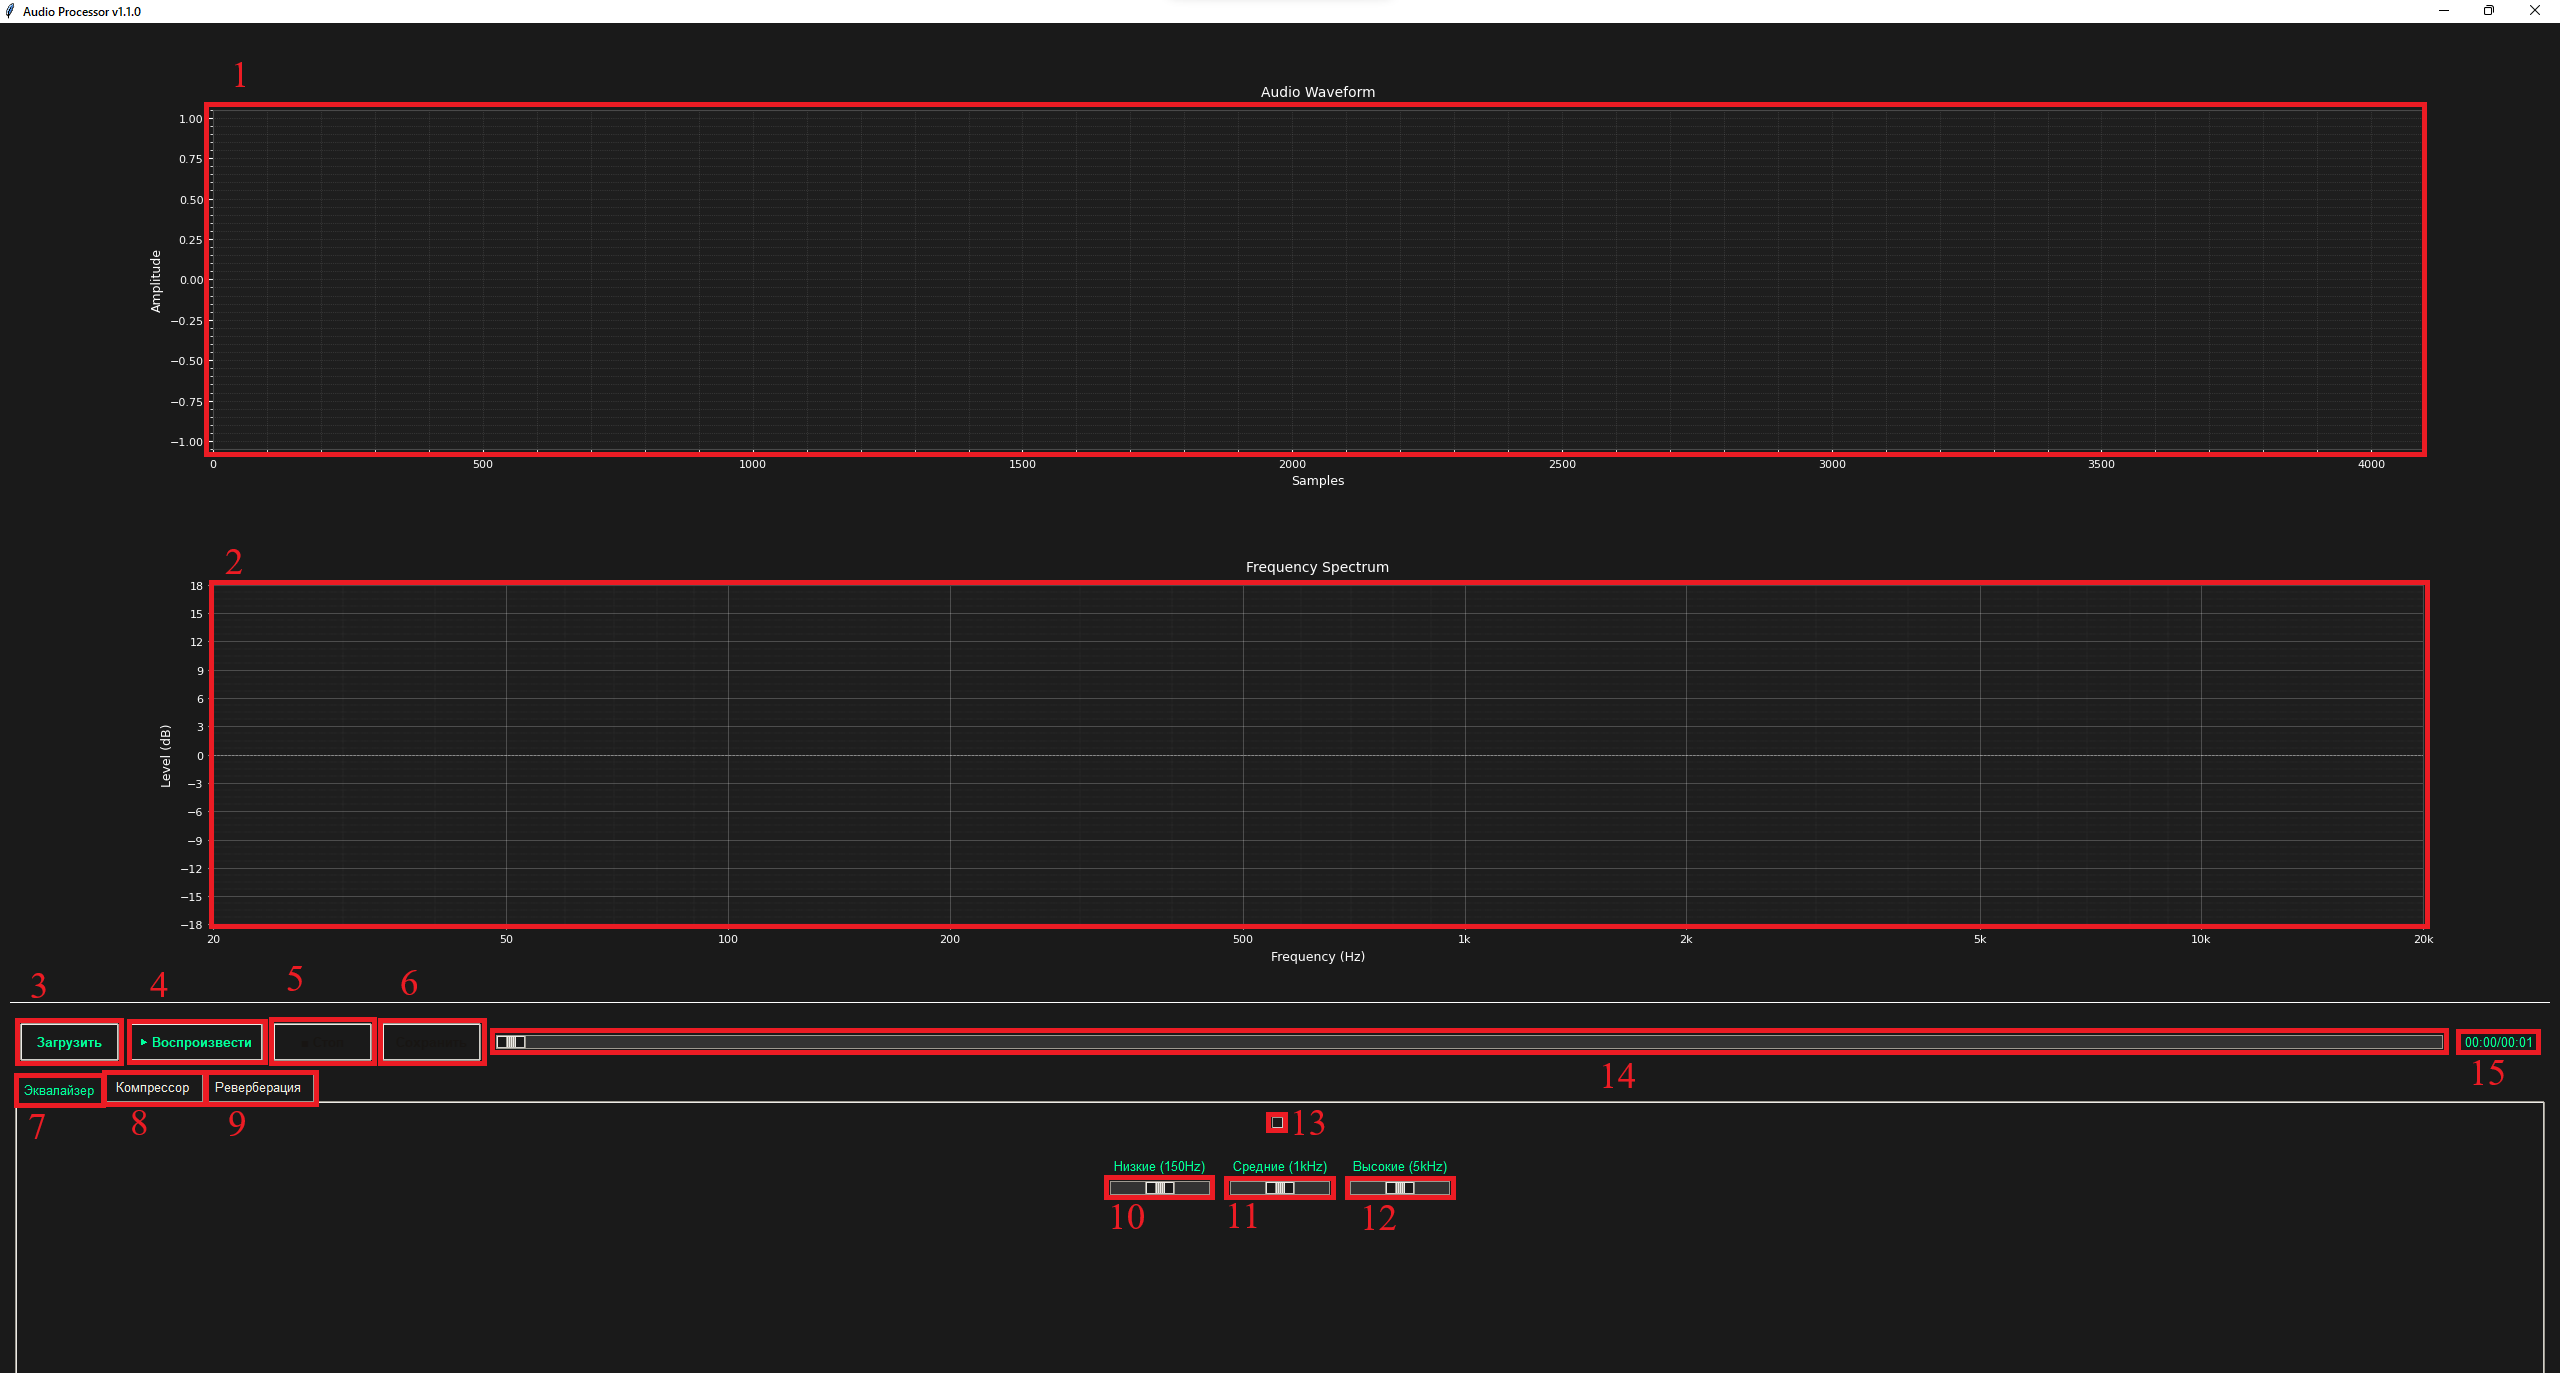
\includegraphics[width=0.8\linewidth]{1}}
	\caption{Макет интерфейса программы}
	\label{1:image}
\end{figure}
\clearpage

На рисунке 3.3 изображён макет вкладки компрессора. Макет содержит следующие элементы:
\begin{enumerate}
	\item Бегунок настройки порогового значения.
	\item Бегунок настройки параметров сжатия.
	\item Бегунок настройки времени атаки в миллисекундах.
	\item Бегунок настройки времени восстановления сигнала в миллисекундах.
	\item Бегунок настройки усиления выходного сигнала.
	\item Чекбокс включения эффека.
\end{enumerate}

\begin{figure}[ht]
	\center{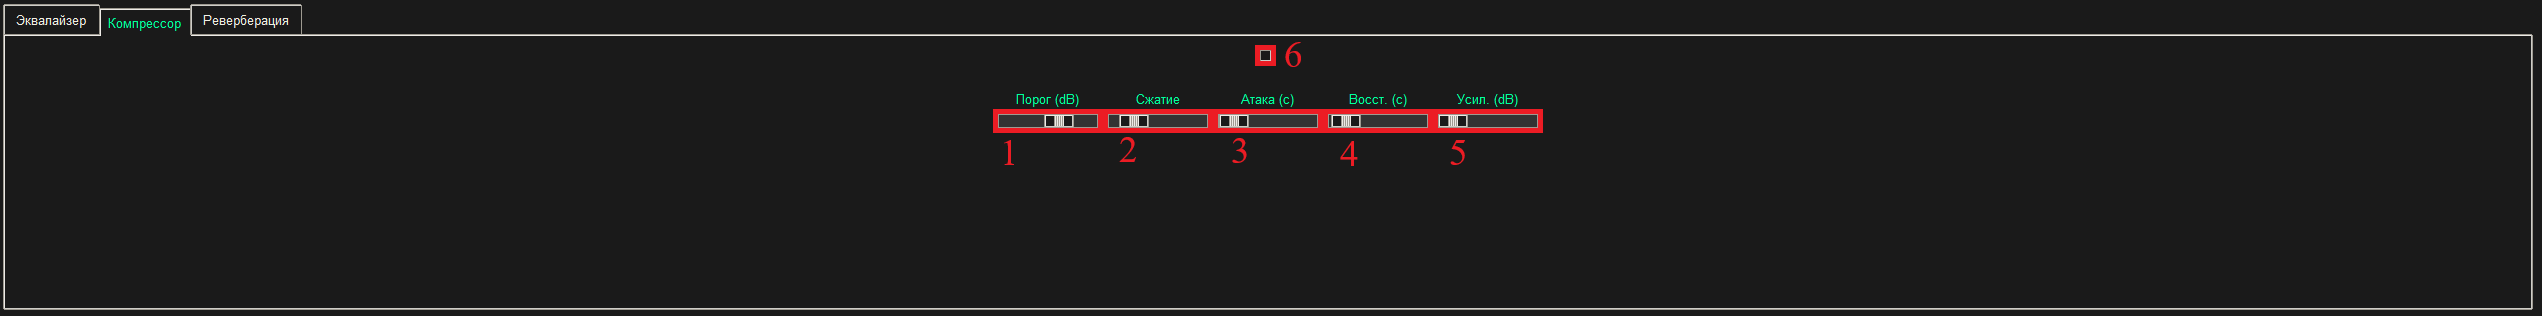
\includegraphics[width=1\linewidth]{2}}
	\caption{Макет окна компрессора}
	\label{2:image}
\end{figure}

На рисунке 3.4 изображён макет вкладки реверберации. Макет содержит следующие элементы:
\begin{enumerate}
	\item Бегунок настройки уровня эффекта.
	\item Бегунок настройки исходного звука.
	\item Бегунок настройки размера пространства.
	\item Бегунок настройки затухания.
	\item Чекбокс включения эффекта.
\end{enumerate}

\begin{figure}[ht]
	\center{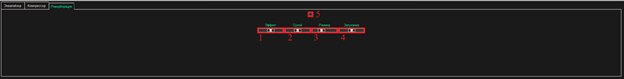
\includegraphics[width=1\linewidth]{3}}
	\caption{Макет окна реверберации}
	\label{3:image}
\end{figure}
\clearpage